\section{Dataset}
\label{dataset}
\begin{figure*}[!h]
  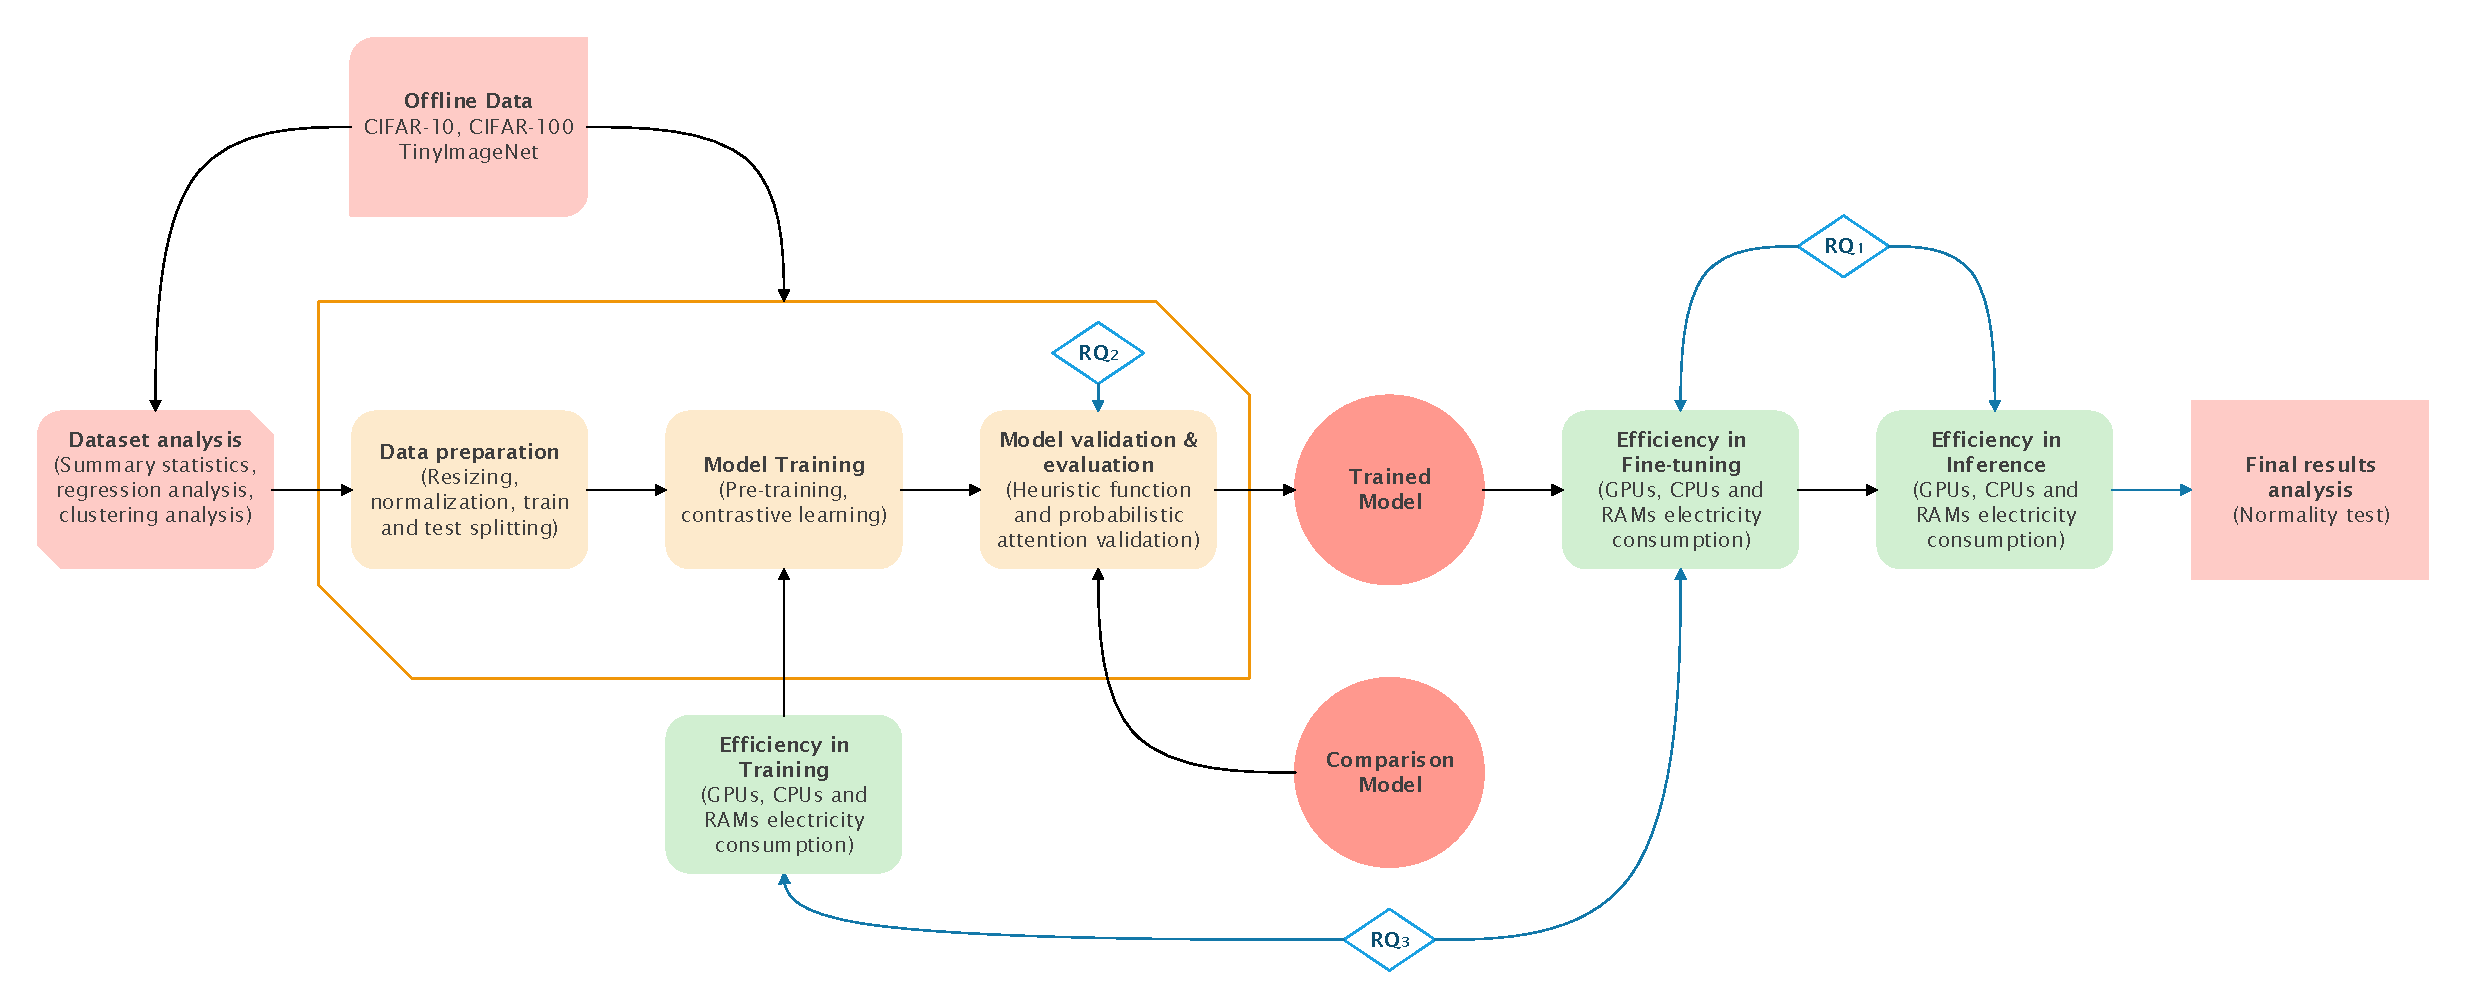
\includegraphics[width=\textwidth]{images/pipeline_final.pdf}
  \caption{Overview of the experiment pipeline}
  \label{pipeline}
\end{figure*}
The selection of a suitable dataset is a critical aspect of training machine learning models. The primary reason for choosing CIFAR-10/100 and TinynImageNet is the computational cost that larger datasets such as ImageNet and JFT-300M requires. These datasets contain a significantly larger number of images, and training on them requires a large amount of computational power and storage capacity. Given our research aim, which is to prove the energy efficiency of our modified Vit architecture, it is not feasible to use these datasets.

The datasets we have used are commonly used to train and evaluate machine learning models, particularly in the field of deep learning. Because the images are relatively small and low-resolution, the datasets can be trained on standard hardware without requiring a large amount of memory or computational resources. Additionally, because the images contain a wide variety of objects and backgrounds, they are a good benchmark for evaluating a model's ability to generalize to new, unseen data.

Over the years, many state-of-the-art models have been trained and evaluated on these datasets, including various convolutional neural network (CNN) and Vision Transformer (ViT) architectures. Achieving high accuracy on these datasets has become a standard benchmark for evaluating the performance of image classification models.

This decision allows us to focus on proving the energy efficiency of our architecture, which is the primary objective of our research.
CIFAR-10, CIFAR-100 are benchmark datasets commonly used for image classification tasks in computer vision research while Tiny ImageNet can give us a good understanding on the generalization capacity of the model. 

CIFAR-10 consists of 60,000 32x32 color images in 10 classes, with 6,000 images per class. The 10 classes are: airplane, automobile, bird, cat, deer, dog, frog, horse, ship, and truck.

CIFAR-100 also consists of 60,000 32x32 color images but divided in 100 classes, with 600 images per class. The 100 classes are grouped into 20 superclasses, each containing 5 subclasses. For example, the "aquatic mammals" superclass contains the "beaver", "dolphin", "otter", "seal", and "whale" subclasses.

Tiny ImageNet is a reduced version of the ImageNet dataset, which is a large-scale image dataset used for training deep learning models for computer vision tasks. The Tiny ImageNet dataset consists of 200 classes, each with 500 training images and 50 validation and test images. The images in this dataset are of size 64x64 pixels, significantly smaller than the images in the original ImageNet dataset.

